\chapter{Floor-fractured craters}
\label{C5-chap6}

\textit{This  chapter is  a  reproduction of  the  paper published  in
  Journal of Geophysical  Research untitled: \textbf{A model  for the dynamics
  of crater-centered  intrusion: Application to  lunar floor-fractured
  craters}} \citep{Thorey:2014cv}.

 \minitoc

\begin{abstract}

  Lunar Floor-Fractured Craters (FFCs) are a class of craters modified
  by post impact  mechanisms. They are defined  by distinctive shallow
  floors that  are convex or  plate-like, sometimes with a  wide floor
  moat bordering  the wall  region.  Radial, concentric  and polygonal
  floor fractures  suggest an endogenous process  of modification. Two
  mechanisms  have been  proposed  to account  for such  deformations:
  viscous relaxation and spreading of a magma intrusion at depth below
  the crater. To test the second assumption and bring more constraints
  on the  intrusion process, we  develop a  model for the  dynamics of
  magma spreading below an elastic  overlying layer with a crater-like
  topography. As predicted in  precedent more qualitative studies, the
  increase in  lithostatic pressure at  the crater wall  zone prevents
  the intrusion from spreading laterally, leading to the thickening of
  the intrusion. Additionally,  our model shows that  the final crater
  floor appearance  after the  uplift, that could  be convex  or flat,
  with or without a circular moat  bordering the wall zone, depends on
  the elastic  thickness of the  layer overlying the intrusion  and on
  the crater size. As a result, our model provides a simple formula to
  derive the elastic  thickness of the layer  overlying the intrusion,
  and hence a  minimum estimate for the intrusion  depth. Finally, our
  model  suggests that  crust  redistribution by  cratering must  have
  controlled magma ascent below most of these craters.

\end{abstract}

\section{Introduction}
\label{C5-Introduction}

A large fraction of the magma produced by mantle melting never reaches
the surface as it intrudes the shallow layers of the planet. On Earth,
the volume of intrusive magma is estimated to be $10$ times (resp. $5$
times) the volume  of extrusive lava for the  continental crust (resp.
the  oceanic  crust)  \citep{Crisp:1984dm}.    Buoyancy  is  the  main
mechanism driving up the magma from the interior to the shallow layers
or the  surface of  the planets.   It has been  shown that  dykes stop
their propagation when they become neutrally buoyant relative to their
surroundings       \citep{Walker:1989jq,Rivalta:2005kd,Taisne:2009va}.
Therefore, the  intrusive to  extrusive ratio  largely depends  on the
respective density of the crust and magma.
	
The density of the lunar crust is particularly low.  The last estimate
from  the GRAIL  NASA  mission provides  for a  mean  density for  the
highlands of  2550 kg.m$^{-3}$,  even lower  than what  was previously
assumed \citep{Wieczorek:2013ipa}.  Both  the light anorthite minerals
that form the lunar crust and impact induced fractures and brecciation
contribute  to its  low  density  \citep{Wilhelms:1987vb}.  Given  the
large  density of  magma inferred  from  the composition  of the  mare
basalts   that    are   generally   rich   in    FeO   and   TiO$_{2}$
\citep{Wieczorek:2001jt}, the intrusive to extrusive ratio on the Moon
might       be       even       higher       than       on       Earth
\citep{ElBaz:1970kc,Wilson:1981fm,Hiesinger:2006cb,Glotch:2010ih}. \citet{Head:1992bk}
estimated an upper limit of $50:1$ for this ratio.  However, there are
no solid  constraints supporting this  estimate and although it  is an
important    parameter    in    lunar   thermal    evolution    models
\citep{Laneuville:2013gp}, it is poorly constrained.
	
Extrusions of lava preferentially  occurred within large impact basins
on the near side of the Moon where a large fraction of the low-density
crust has been removed. However, the  trajectory of the magma from its
source  to the  surface  is  unknown. The  magma  could have  ascended
directly  from the  source  to  the surface  \citep{Wieczorek:2001jt};
alternatively,  it might  have first  accumulated at  the crust-mantle
interface   before    erupting   where    the   crust    was   thinner
\citep{Wilson:1981fm}.
	
Possible sites  for intrusions on  the Moon are  below floor-fractured
craters   (FFCs).     These   craters   have   been    identified   by
\citet{Schultz:1976kt}; they have shallow  floors with a plate-like or
convex  appearance,  wide  floor  moats  and  radial,  concentric  and
polygonal  floor  fractures.   \citet{Schultz:1976kt}  has  classified
about  200  FFCs.    Similar  FFCs  have  been   observed  on  Mercury
\citep{Head:2008cm},                                              Mars
\citep{Schultz:1978tw,Schultz:1979iw,Sato:2010ex}       and      Venus
\citep{Wichman:1995ju}.  The  database and classification  proposed by
\citet{Schultz:1976kt}     have    recently     been    updated     by
\citet{Jozwiak:2012dq} who used new data  from the Lunar Orbiter Laser
Altimeter (LOLA)  and Lunar Reconnaissance Orbiter  Camera (LROC). The
deformations affecting  these craters are contained  within the crater
interior.  Two mechanisms  have been proposed to  explain the features
observed at FFCs: 1) spreading of  a magmatic intrusion at depth below
the                            crater                            floor
\citep{Schultz:1976kt,Wichman:1993hk,Wichman:1995ic,Wichman:1996bj,Jozwiak:2012dq}
and  2) viscous  relaxation of  the crater  floor induced  by a  local
thermal gradient  caused by the impact  \citep{Hall:1981kl}.  However,
viscous  relaxation   of  the  crater   floor  has  been   modeled  by
\citet{Dombard:2001gs} but, for typical  elastic parameters, the lunar
crust is too rigid and shallowing  of craters smaller than $100$ km is
not significant.  Hence, if the deformations observed at FFCs resulted
indeed  from   magmatic  intrusion,  they  might   give  us  important
constraints  and clues  on the  process of  magmatic intrusion  in the
lunar crust.
	
The classical,  static, model of laccoliths  of \citet{Pollard:1973ho}
has  previously  been applied  to  the  case  of  FFCs to  deduce  the
intrusion          depth          and          magma          pressure
\citep{Wichman:1993hk,Wichman:1996bj,Jozwiak:2012dq}.  In  this static
model, the intrusion radius is known  a priori. The intrusion shape is
controlled by the  elastic deformation of a thin elastic  layer on top
of the laccolith and the  elastic pressure necessary for deforming the
overlying  layer  is  assumed  to be  equilibrated  by  magma  weight.
However, \citet{Michaut:2011kg}  and \citet{Bunger:2011cb}  have shown
that, if the  elastic deformation of the overlying  layer controls the
flow shape  and its dynamics during  a first spreading phase,  the own
weight of  the flow becomes dominant  during a second phase  where the
flow shape  shows a flat top.   Furthermore, in all these  models, the
possible  effect of  a  thickening  of the  overlying  layer has  been
ignored.
	
Here, we modify  the model proposed by  \citet{Michaut:2011kg} for the
dynamics  of a  magma intrusion  below an  elastic overlying  layer in
order to account for the effects of the crater topography, i.e. for an
overlying layer of  variable thickness.  We show  that different types
of  deformations  of  the  crater floor  are  expected,  as  initially
predicted by  \citet{Schultz:1976kt}, and  that they mainly  depend on
the elastic thickness of the layer  overlying the intrusion and on the
crater size.

\section{Floor-fractured craters}
\label{C5-FFC}

Floor-fractured  craters are  craters that  have undergone  endogenous
deformations  after the  impact.  About  two hundreds  FFCs have  been
observed on the Moon and precisely described by \citet{Schultz:1976kt}
who studied their structure and geology using Lunar Orbiter and Apollo
stereo sets.  \citet{Schultz:1976kt} proposed  a classification into 6
categories based on their sizes, morphological features and degrees of
modification;  classification  which  has  recently  been  updated  by
\citet{Jozwiak:2012dq} using the Lunar  Orbiter Laser Altimeter (LOLA)
and Lunar Reconnaissance Orbiter Camera (LROC) (Table \ref{C5-tab1}).

\begin{figure}[h!]
  \graphicspath{ {/Users/thorey/Documents/These/Submission/Article/FFC_JGR_2013/Paper_APRES_2nd_REVIEW/} }
  \begin{center}
    \includegraphics[scale=0.75]{fig5-1.eps}
    \caption{\textbf{a)}   Class  2   floor-fractured  crater   Briggs
      ($26.5^{\circ}$N,$69.1^{\circ}$W),   $37$    km   in   diameter:
      \textbf{Left},  high resolution  scan  from  USGS Lunar  Orbiter
      Digitization Project. \textbf{Center}, topographic map extracted
      from LOLA  data. Latitudes and  longitudes are indicated  on the
      figure.  Color  scale indicates  the topography in  meters.  The
      scale  origin  is  given  by   the  zero  level  of  the  geoid.
      \textbf{Right},  at  the  top,  Northwest-Southeast  topographic
      profile extracted from  line a) on the  central topographic map,
      at the bottom, Southwest-Northeast topographic profile extracted
      from line b)  on the central topographic  map.  \textbf{b)} Same
      plots      for       the      class      3       FFC      Warner
      ($4.0^{\circ}$S,$87.3^{\circ}$E) that is 35 km in diameter.}
    \label{C5-fig5-1}
  \end{center}
\end{figure}
	
Radial and concentric fracture networks  generally cross the floors of
these  craters \citep{Schultz:1976kt}.   Another  striking feature  of
FFCs  is their  shallow  floors: except  for class  1  FFCs, they  all
exhibit a  significant shallowing  of their  floors compared  to fresh
craters the same size \citep{Schultz:1976kt,Jozwiak:2012dq}.
	
Floor uplift  mainly results  in two different  modes of  crater floor
appearance \citep{Schultz:1976kt}.   In particular, FFCs of  classes 3
and  5 show  a flat  central  floor, characteristic  of a  piston-like
uplift of  the crater floor;  additionally, a large  circular U-shaped
moat adjacent to the wall zone borders  the flat floor of class 3 FFCs
\citep{Schultz:1976kt,Jozwiak:2012dq}. A typical example  of a class 3
FFC is the crater Warner, which is 35 km in diameter and is located at
$4.0^{\circ}$S,  $87.3^{\circ}$E  in the  southern  part  of the  Mare
Smythii (Figure \ref{C5-fig5-1} b). In contrast, the floors of craters
of classes 2 and 4 appear  convex, indicating a different mechanism of
crater floor uplift  \citep{Schultz:1976kt,Jozwiak:2012dq}.  Briggs is
a good archetype of  class 2 FFC, it is a crater of  37 km in diameter
and  is located  at $26.5^{\circ}$N,  $69.1^{\circ}$W, in  the western
part of  the Oceanus  Procellarum (Figure \ref{C5-fig5-1}  a). Craters
showing a convex  floor may also exhibit moats adjacent  to their wall
zone but these are  V-shaped; this is the case for  classes 4a, 4b and
4c FFCs. In  addition, craters of class 4b also  exhibit an inner wall
zone.



\begin{table}
  \caption{A summary of Floor-Fractured Craters classification as proposed by \citet{Jozwiak:2012dq} following \citet{Schultz:1976kt}}
  \centering
  \begin{tabular}{c|c}
    \hline
    Class & Description \\
    \hline

    1 & Large craters: $50-300$ km (average $140$ km)\\
          & Deep floor \\
          & Absence of moats\\
          & Radial or concentric fractures\\
    \hline
    2 & Mid-size craters: $13-75$ km (mean $30$ km)\\
          & Shallow convex floor \\
          & Absence of moats\\
          & Strong concentric fractures\\
    \hline
    3 & $12-170$ km (mean $50$ km)\\
          & Shallow central flat floor\\
          & Wide U-Shaped moat\\
          & Radial or polygonal fractures\\
    \hline
    4a & Small craters: $4-38$ km (mean $15$km)\\
          & Shallow convex floor \\
          & Weak V-shaped moat\\
          & Strong radial and concentric fractures \\
    \hline
    4b & Small craters: $7-45$ km (average:$25$km)\\
          & Shallow convex floor \\
          & Pronounced V-shaped moat + inner ridges\\
          & Subtle radial fractures\\
    \hline
    4c & Small craters: average $15$ km \\
          & Flat or concave up floor \\
          & V-shaped moats \\
          & Hummocky, lack of fracture \\
    \hline
    5 & Large craters: $12-177$ km (average $70$km)\\
          & Shallow old and degraded central flat floor\\
          & Absence of moats \\
          & Strong radial, concentric and/or polygonal fractures\\
    \hline
    6 & Large craters: $50-200$km \\
          & Completely flooded by basalt\\
          & Absence of moats\\
          & Concentric fractures
            \label{C5-tab1}
  \end{tabular} 
  % \tablenotetext{a}{Footnote text here.}
\end{table}
	
	
Finally, class 1  FFCs show only limited deformations  while the floor
of class 6 FFCs has been flooded by mare lavas, illustrating the close
relationship  between  magmatism  and deformations  at  these  craters
\citep{Schultz:1976kt,Jozwiak:2012dq}.

\section{An  axisymmetric model  for  a  magmatic intrusion  spreading
  below a crater-like topography}

In this model, we consider  the spreading of an axisymmetric intrusion
above  a  rigid  layer  and  below  a  thin  overlying  layer  with  a
crater-like topography.
	
\subsection{Crater topography and overlying layer characteristics}
\label{C5-Crater_Topography}
	
On  the Moon,  fresh impact  craters have  been classified  into three
categories according  to their  shapes following crater  formation and
collapse:    simple    craters,    complex    craters    and    basins
\citep{Pike:1974ux,Schultz:1976vl,Pike:1980eh,Baker:2011kh}.    Simple
craters are  bowl-shaped craters that  do not exhibit  any slope-break
\citep{Pike:1980eh}.    With  increasing   diameter,  impact   craters
transition to complex craters that  are characterized by an inner flat
floor, terraced rims  and a central peak. On the  Moon, the transition
from simple  to complex craters occurs  at a diameter of  $\sim 15$ km
\citep{Pike:1980eh,Hiesinger:2006cb,OKeefe:1999uj,Kalynn:2013fg}.
Although not all  do, most craters larger than $100$  km exhibit rings
on    their    flat    floors    and    are    defined    as    basins
\citep{Wilhelms:1987vb,Schultz:1988wb}.   In  our  model,  we  do  not
consider basins  and study  the spreading of  a magmatic  intrusion at
depth below simple and complex craters.

\begin{figure}[h!]
  \graphicspath{ {/Users/thorey/Documents/These/Submission/Article/FFC_JGR_2013/Paper_APRES_2nd_REVIEW/} }
  \centering
  \noindent\includegraphics[scale=0.75]{fig3-1.eps}
  \caption{ Here, we show the two normalized sigmoid function $\xi(r)$
    used to  parameterize the two end-member  crater topographies (see
    Section  \ref{C5-Crater_Topography}).    \textbf{a)}  The  sigmoid
    function    of    a    simple     crater    is    modeled    using
    $D_c/4\alpha C=\zeta=0.25$.  \textbf{b)} The sigmoid function of a
    complex crater is modeled using $D_c/4\alpha C=\zeta=0.13$. }
  \label{C5-fig3-1}
\end{figure}
	
In this model, we account for  the effects of the crater topography on
the intrusion  dynamics.  The normalized sigmoid  function $\xi(r)$ is
used to parameterize the crater topography
\begin{equation}
  \xi(r)=\frac{1}{1+e^{-\frac{4\alpha(r-C)}{D_c}}}-\frac{1}{1+e^{\frac{4\alpha C}{D_c}}}
  \label{C5-3-3}
\end{equation}	
where $D_c$ is the intrusion depth,  $C$ the crater radius, defined as
the distance  from the crater center  to the center of  the wall zone,
and   $\alpha$  the   average   slope  of   the   wall  zone   (Figure
\ref{C5-fig3-1}).  The  elevation in  height relatively to  the crater
center, i.e the crater topography, is then given by
\begin{equation}
  T_p(r)=D_c\xi(r)
  \label{C5-topo}
\end{equation}
and results in an increase in  lithostatic pressure at the crater wall
zone.
	
For  simple  craters,   our  definition  of  the   crater  radius  $C$
corresponds    to    half    of   the    observed    crater    radius.
\citet{Pike:1980eh}  shows  that  the   average  wall  slope  $\alpha$
increases gradually from about $0.3$ ($19^{\circ}$), for craters $0.5$
km  in  diameter, to  $0.4$  ($25^{\circ}$)  for  craters $15$  km  in
diameter \citep{Kalynn:2013fg}.  To model a simple crater, we thus use
$D_c/4\alpha C  =0.25$ (Figure \ref{C5-fig3-1} a),  which, for $C=2.5$
km and $\alpha=0.4$ ($25^{\circ}$) gives  a corresponding $D_c$ of $1$
km in  agreement with  \citet{Pike:1980eh}.  For complex  craters, the
size  of the  central flat  floor,  relatively to  the crater  radius,
increases from $25  \%$, for a crater  20 km in diameter,  to $50 \%$,
for a crater that is $100$ km crater in diameter.  The wall of complex
craters exhibits  walls at  the angle  of repose  ($\sim 30^{\circ}$),
terraces, and hilly toes that combine to form a wall zone of effective
slope  value  that  decreases  from $\alpha=  0.5$  ($30^{\circ}$)  to
$\alpha=0.2$ ($12^{\circ}$) as the crater diameter increases from $20$
to $100$ km \citep{Pike:1980eh,Bray:2008fu,Kalynn:2013fg}.  To model a
complex  crater,   we  use   a  ratio  $D_c/4\alpha   C=0.13$  (Figure
\ref{C5-fig3-1}  b) which,  for $C=14$  km and  $\alpha=0.4$, i.e.   a
crater that is $40$ km in diameter, gives $D_c=3$ km in agreement with
\citet{Pike:1980eh} and \citet{Kalynn:2013fg}.
	 
Impact  induces  fracture and  brecciation  beneath  the crater  floor
\citep{Wilhelms:1987vb,Melosh:1989jl,Jolliff:2000vf}  and also  causes
melting        and        compaction        of        the        pores
\citep{Melosh:1989jl,Schultz:1976kt}.  If the melting during impact is
negligible and the neutral buoyancy zone of the magma lies immediately
beneath   an  impact   brecciated   lens,  as   is  commonly   assumed
\citep{Schultz:1976kt,Wichman:1996bj,Jozwiak:2012dq},   the  overlying
layer  would not  respond  elastically  due to  its  lack of  coherent
structure. We consider the case of a strengthless overlying layer with
a  crater   like  topography  given  by   (\ref{C5-topo})  in  Section
\ref{C5-Strengthless_Layer1}.   However, a  coherent impact  melt unit
commonly     stands    on     top    of     the    brecciated     lens
\citep{Melosh:1989jl,Schultz:1976kt}.   The neutral  buoyancy zone  of
the magma  depends on the  crust and magma  density and could  also be
situated deeper than the bottom of  the brecciated lens.  As a result,
the overlying layer would deform  elastically above the intrusion.  In
our model,  we thus consider  the case of  an overlying layer  with an
elastic thickness  $T_e(r)$ that varies  with radial coordinate  r and
thickens  at  the  crater  wall zone  (Figure  \ref{C5-fig3-2}).   The
elastic  layer  is  characterized  by  a Young's  modulus  $E$  and  a
Poisson's ratio $\nu$.   For simplicity, the thickness  of the elastic
layer, showing a simple or  a complex crater topography, is considered
to be equal to the intrusion depth and is given by
\begin{equation}
  T_e(r)=T_{e}^0(1+\Psi \xi(r))
  \label{C5-3-2}
\end{equation}	
where $\Psi=D_{c}/T_{e}^0$ is the ratio of the crater depth $D_{c}$ to
the  intrusion depth  at the  center $T_{e}^0$  and characterizes  the
thickening of the  upper elastic layer at the crater  wall zone.  As a
result of  this assumption, the  intrusion depth is  underestimated in
the model, but  if a constant thickness brecciated  layer overlies the
intrusion and  underlies such an elastic  layer, it does not  have any
effect on the intrusion dynamics.  The crater topography $T_p$ is then
given by
\begin{equation}
  T_p(r)=T_e(r)-T_e^0=T_e^0\Psi\xi(r)=D_c\xi(r).
  \label{C5-topo1}
\end{equation}
	 
Central  peaks   are  common  features  of   complex  craters.   Their
dimensions depend on both projectile  and target properties as well as
on  the  impact  angle  \citep{Schultz:1994cv,Bray:2008fu}.   However,
their width can reach  one fourth of the crater floor  and they can be
as high  as half  of the  crater depth; hence  such a  structure could
influence the intrusion dynamics.  The effect of a central peak on the
spreading  of  an intrusion  is  examined  in Appendix  \ref{chap:A4}.
Moreover, a raised  rim, uplifted relative to  the pre-impact surface,
is  usually  present   at  the  exterior  of  the   crater  wall  zone
\citep{Pike:1976ei,Pike:1980eh}. Although,  for simplicity, we  do not
model the effect of this feature, we discuss its possible influence on
intrusion emplacement in Section \ref{C5-InjectionRateDiscussion}.
	 		 
\subsection{Equations of Motion}
	
We assume that the flow spreads along a thin bedding plane and neglect
fracturing  at the  tip.   The  magma is  considered  to  behave as  a
newtonian  fluid   with  a   constant  viscosity  $\mu$   and  density
$\rho_{m}$.   The  intrusion is  fed  at  a  constant rate  through  a
cylindrical conduit of  diameter $a$.  The vertical  coordinate $z$ is
oriented upward (Figure \ref{C5-fig3-2}).

\begin{figure}[h!]
  \graphicspath{ {/Users/thorey/Documents/These/Submission/Article/FFC_JGR_2013/Paper_APRES_2nd_REVIEW/} }
  \begin{center}
    \includegraphics[width=0.9\columnwidth]{fig3-2.eps}
    \caption{Sketch of the intrusion  spreading below an impact crater
      topography.  $D_{c}$  (resp.  $C$) represents the  initial depth
      (resp. radius) of the impact crater. The intrusion spreads above
      a rigid  homogeneous and horizontal bedrock  at depth $T_{e}(r)$
      below the  crater floor. At  the center, the intrusion  depth is
      noted $T_{e}^0$.}
    \label{C5-fig3-2}
  \end{center}
\end{figure}
 	
\subsubsection{Momentum equation}
\label{C5-Equation_Momentum}
	
The dynamics of the flow is given by the solution of the Navier-Stokes
equation in  cylindrical geometry.  The  magma has a  relatively large
viscosity, hence the flow is in a laminar regime and the inertia terms
can  be  neglected.   The  intrusion  develops  over  a  length  scale
comparable to the  crater size that is much larger  than its thickness
$H$  ($C>>H$),   hence  the  lubrication  assumption   allows  further
simplifications       \citep{Huppert:1982a,Michaut:2009jx}.        The
Navier-Stokes equations in  the radial and vertical  directions for an
axisymmetric, incompressible flow of newtonian fluid resume to
\begin{eqnarray}
  -\frac{\partial P}{\partial r} + \mu \frac{\partial^{2}u}{\partial z^{2}} &=&0\label{C5-eq4} \\
  -\frac{\partial P}{\partial z} - \rho_{m}g& =&0.
                                                 \label{C5-eq5}
\end{eqnarray}

Integration of (\ref{C5-eq5}) gives the pressure within the flow
\begin{equation}
  P(r,t)=\rho_{m}g(h(r,t)-z) + \rho_{c}gT_e(r) + P_{e}(r,t)
  \label{C5-eq6}
\end{equation}
where  $h(r,t)$  is  the  intrusion  thickness  and  $\rho_c$  is  the
overlying layer density.   The pressure is the sum  of three different
contributions: the weight of the magma  and of the overlying layer and
the elastic  pressure $P_e$  due to the  deformation of  the overlying
elastic  layer. In  the absence  of radial  forces within  the elastic
plate, the elastic pressure required for bending the plate is given by
the force per unit area that  is necessary for a vertical displacement
$h$ of the thin elastic plate \citep{Turcotte:1982ca}
\begin{equation}
  P_{e}(r,t)=\nabla^{2}_{r}\left( D(r)\nabla^{2}_{r}h(r) \right) \\	
  \label{C5-eq8}	
\end{equation}
where
\begin{equation}
  D(r)=\frac{ET_e(r)^{3}}{12(1-\nu^2)}
  \label{C5-eq8a}
\end{equation}
is the  flexural rigidity of  the plate  which depends on  the elastic
layer thickness  $T_{e}(r)$, Young's  modulus $E$ and  Poisson's ratio
$\nu$.
	 	
Substituting (\ref{C5-eq6}) and (\ref{C5-eq8}) into (\ref{C5-eq4}) and
integrating twice  using no-slip  boundary conditions  at the  top and
bottom of the  intrusion, i.e. $u_{z=0}=u_{z=h}=0$, we  get the radial
velocity within the flow
\begin{equation}
  u(r,z,t)= \frac{1}{2\mu}\left(\rho_{m}g \frac{\partial h(r,t)}{\partial r} + \rho_{c}g \frac{\partial T_e(r)}{\partial r}+\frac{\partial}{\partial r}\left ( \nabla^{2}_{r}(D(r)\nabla^{2}_{r}h(r,t))\right)\right) (z^{2}-zh(r,t))
  \label{C5-eq10}
\end{equation}

\subsubsection{Injection rate}
\label{C5-Injection_Rate}

Assuming a Poiseuille flow within the cylindrical feeding conduit, the
vertical  injection velocity  $w(r,t)$  and injection  rate $Q_0$  are
given by:
\begin{equation*}
  w(r,t)=
  \begin{cases}
    \frac{ \Delta P}{4 \mu Z_{c}} (\frac{a^{2}}{4}-r^{2})& r \le \frac{a}{2}\\
    0 & r > \frac{a}{2}
  \end{cases}
  \label{C5-eq12}
\end{equation*}
\begin{equation}
  Q_{0}=\frac{\pi \Delta P a^{4}}{128 \mu Z_c}
  \label{C5-eq11}
\end{equation}
where  $\Delta P$  is  the  initial overpressure  within  the melt  at
$z=Z_{c}$.

\subsubsection{Final equation}
\label{C5-Final_Equation}

To obtain  the final  equation of motion,  we write  mass conservation
integrated over the flow thickness:
\begin{equation}
  \frac{\partial h(r,t)}{\partial t} = -\frac{1}{r} \frac{\partial}{\partial r} \left( r \int_{0}^{h(r,t)} u(r,z,t) dz\right ) + w(r,t) 
  \label{C5-eq15}
\end{equation}
Injecting  (\ref{C5-eq10})   into  (\ref{C5-eq15})   and  substituting
$T_{e}(r)$  by (\ref{C5-3-2})  gives  the evolution  equation for  the
intrusion thickness $h$:
\begin{eqnarray}
  \frac{\partial h}{\partial t} &=&\frac{\rho_{m}g}{12 \mu} \frac{1}{r} \frac{\partial}{\partial r}\left (r h^{3} \frac{\partial h}{\partial r} \right)+ \frac{\rho_{c}g\Psi T_{e}^0}{12 \mu} \frac{1}{r} \frac{\partial}{\partial r}\left ( r h^{3} \frac{\partial \xi(r)}{\partial r}\right ) \nonumber \\
                                &+&\frac{E T_{e}^{0^{3}}}{144\mu (1-\nu^{2})}\frac{1}{r}\frac{\partial}{\partial r}\left ( r h^{3} \frac{\partial}{\partial r} \left(\nabla^{2}_{r} ((1+\Psi \xi(r))^{3}\nabla^{2}_{r}h )\right)\right )+ w(r,t) 
                                    \label{C5-eq16}
\end{eqnarray}
As  expected,  this evolution  equation  accounts  for four  different
contributions.   The first  term  on the  right  hand side  represents
gravitational  spreading  of  the  intrusion; except  for  a  constant
arising from a no-slip boundary at the top of the flow, it is the same
as for a gravity current  \citep{Huppert:1982a}. This term is negative
and induces  magma spreading. The  second term is associated  with the
increase  in  lithostatic  pressure  at   the  crater  wall  zone  and
represents the lithostatic barrier the flow has to face when spreading
below  the crater  wall zone;  it is  not present  in the  case of  an
overlying  layer of  constant thickness  \citep{Michaut:2011kg}.  This
term is positive  and opposes to the flow.  The  third term represents
squeezing of  the flow in response  to the elastic deformation  of the
overlying layer.  This  term is negative and induces  spreading in the
case    of     an    elastic     layer    of     constant    thickness
\citep{Michaut:2011kg}. However, in the case  of a layer that thickens
with  $r$, it  can  become positive  and  oppose to  the  flow if  the
thickening is rapid  and important, i.e. at the crater  wall zone. The
last term represents the injection rate.

\subsection{Nondimensionalization}
\label{C5-Dimensionless_Equation}

Because the  model depends  on a  large set  of parameters  (see Table
\ref{C5-tab2}), we nondimensionalize the flow equation (\ref{C5-eq16})
using    the   crater    radius   $C$,    as   defined    in   Section
\ref{C5-Crater_Topography},  as the  characteristic  length scale,  as
well as a height scale $H$ and a time scale $\tau$ given by
\begin{equation}
  \label{C5-eq18}
  H= \left (\frac{12\mu Q_{0}}{\rho_{m}g \pi}\right ) ^{\frac{1}{4}}=a\left( \frac{3 \Delta P}{32\rho_{m}gZ_{c}}\right ) ^{\frac{1}{4}}
\end{equation}
\begin{equation}
  \tau=\frac{\pi C^{2} H}{Q_{0}}=\left (\frac{12\mu}{\rho_{m}g \pi}\right)^{\frac{1}{4}}\pi C^{2}Q_{0}^{-\frac{
      3}{4}}\label{C5-eq19}
\end{equation}
The  height scale  and  the time  scale are  defined  by equating  the
nondimensional group in front of the  gravity current term to 1, i.e.,
$(\tau \rho_{m}gH^{3})/(12\mu  C^{2})=1$. The height scale  $H$ is the
characteristic   height    scale   of    a   gravity    current   flow
\citep{Huppert:1982a}. $\tau$ is the time  scale for a gravity current
to fill in the crater; it mainly depends on the injection rate. In the
case  of   an  upper   layer  with   constant  thickness   $T_e^0$,  a
characteristic length  scale for  the flow  is the  flexural parameter
$\Lambda$, as defined by \citet{Turcotte:1982ca}, given by
\begin{equation}
  \Lambda=\left( \frac{E T_{e}^{0^{3}}}{12 (1-\nu^{2})\rho_{m}g} \right )^{\frac{1}{4}}
  \label{C5-eq99}
\end{equation}
it  represents  the wavelength  over  which  the upper  layer  deforms
elastically. However, in this problem, the crater radius $C$ imposes a
horizontal length  scale to the  flow, as the lithostatic  barrier the
flow faces  at the  wall zone  imposes a  limitation to  the intrusion
spreading.   The choice  of  $C$  as the  length  scale  is then  more
relevant. Variables are then written as:
\begin{equation}
  r=Cr^{*} \hspace{0.5cm}h=Hh^{*} \hspace{0.5cm} t=\tau t^{*} 
  \label{C5-eq20}
\end{equation}
where  $r^{*},h^{*}$   and  $t^{*}$  are  the   dimensionless  radius,
thickness and time.  Substituting (\ref{C5-eq20}) into (\ref{C5-eq16})
and dropping the stars, we  finally get the dimensionless equation for
the flow:

\begin{eqnarray}
  \frac{\partial h}{\partial t}&=&\frac{1}{r} \frac{\partial}{\partial r}\left (rh^{3} \frac{\partial h}{\partial r} \right)+ \Xi \frac{1}{r} \frac{\partial}{\partial r}\left ( rh^{3}\frac{\partial \xi(r)}{\partial r}\right )\nonumber\\
                               &+&\Theta \frac{1}{r}\frac{\partial}{\partial r}\left ( rh^{3} \frac{\partial}{\partial r} \nabla^{2}_{r}\left ((1+\Psi \xi(r))^{3}\nabla^{2}_{r}h \right )\right)+ \frac{32}{\gamma^{2}} \left(\frac{1}{4}-\frac{r^{2}}{\gamma^{2}}\right)
                                   \label{C5-eq21}
\end{eqnarray}
where $\xi(r)$ is also made dimensionless
\begin{equation}
  \xi(r)=\frac{1}{1+e^{-\frac{(r-1)}{\zeta}}}-\frac{1}{1+e^{\frac{1}{\zeta}}}\label{C5-eqqqq}
\end{equation}

and  where $\gamma$,  $\zeta$,  $\Xi$, $\Psi$  and  $\Theta$ are  five
dimensionless numbers that control the dynamics of the flow.
\begin{eqnarray}
  \label{C5-Dimensionless1}
  \gamma&=&\frac{a}{C} \label{C5-n1}\\
  \zeta&=&\frac{D_c}{4\alpha C}\label{C5-n2}\\
  \Xi&=& \left(\frac{\rho_{c}gD_{c}}{\rho_{m}gH}\right )\label{C5-n3}\\
  \Psi&=&\frac{D_{c}}{T_{e}^0}\label{C5-n4}\\
  \Theta&=&\left ( \frac{\Lambda}{C} \right )^{4}\label{C5-n5} 
\end{eqnarray}
The  number $\gamma$  represents the  dimensionless source  width. The
number $\zeta$  is four times  the normalized crater wall  zone width;
its    range   of    values    has   been    discussed   in    Section
\ref{C5-Crater_Topography}.  The number $\Xi$ is the ratio between the
lithostatic  pressure  increase  at  the  crater  wall  zone  and  the
hydrostatic  pressure due  to a  magma column  of thickness  $H$.  The
number $\Psi$  is the  dimensionless thickening  of the  upper elastic
layer   at   the  crater   wall   zone,   as  described   in   Section
\ref{C5-Crater_Topography}.   Finally,  the  number  $\Theta$  is  the
dimensionless flexural wavelength  of the upper layer  elevated to the
power  $4$; it  quantifies the  length  scale over  which the  elastic
deformation is effective relative to the crater radius.
	
Additionnally, we define a last dimensionless number $\Omega$
\begin{equation}
  \Omega=\frac{\rho_m}{\rho_c}
\end{equation}
which is the  ratio between the magma and crust  density. The value of
$\Omega$ is set  equal to $1.2$. The dimensionless  topography is then
given by:
	
\begin{equation}
  T_p(r)=\Xi\Omega\xi(r)
  \label{C5-TopoFinal}
\end{equation}

To obtain the crater floor appearance in the different figures, we add
to the  dimensionless expression of the  topography, the dimensionless
thickness $h(r)$ of the intrusion.
	 
	
\subsection{Range of values for the dimensionless numbers}
\label{C5-Dimensionless_Number}
	 
For a conduit  diameter varying between $10$ and $100$  m and a crater
radius between $10$ and $50$  km, the normalized source width $\gamma$
(\ref{C5-n1})   varies   between   $10^{-5}$  and   $10^{-2}$   (Table
\ref{C5-tab3}).  Its  variation does  not significantly  influence the
results and in particular, does not play on the shape of the intrusion
\citep{Michaut:2011kg} ;  it is  fixed at  a value  of $0.02$  in this
study. For  a Young's modulus between  $1$ and $10$ GPa,  a gravity of
$1.62$ m.s$^{-2}$, a magma density  $\rho_m$ between $2800$ and $3200$
kg.m$^{-3}$ and an elastic thickness $T_e^0$ ranging from $0.5$ to $5$
km, the  flexural wavelength  of the upper  layer $\Lambda$,  given by
($\ref{C5-eq99}$),   varies   between   $1$   and   $12$   km   (Table
\ref{C5-tab2}).   Accordingly, for  complex craters  between $20$  and
$100$ km in diameter, our length scale  $C$ is between $6$ km and $40$
km  and the  number $\Theta$  takes values  between $10^{-7}$  and $1$
(Table \ref{C5-tab3}).  For simple craters between $10$ and $20$ km in
diameter, the number $\Theta$ is between $10^{-3}$ and $10$.

\begin{table}[h!]
  \caption{Range of values for the model parameters}
  \centering
  \begin{tabular}{c|c|c}
    \hline
    Parameters& Symbol & Range of values \\
    \hline
              &&\\
    Depth of intrusion & $T_{e}^0$ & $0.5-5$ km \\
    Young's Modulus & $E$ & $1-10$ GPa \\
    Poisson's ratio & $\nu$ & $0.25$ \\
    Gravity & $g$ & $1.62$ m.s$^{-2}$ \\
    Magma density & $\rho_{m}$ & $2800-3200$ kg.m$^{-3}$ \\
    Magma viscosity & $\mu $ & $1-10^{4}$ Pa.s -\\
    Feeder dyke width & $ a$ & $10-100$ m \\
    Depth of the melt source & $Z_{c}$ & $ 200-500$ km \\ 
    Initial overpressure & $\Delta P$ & $1-20$ MPa \\
    Injection rate & $Q_{0}$ &$0.1-2.10^8$ m$^{3}$.s$^{-1}$ \\
    Crust density & $\rho_{c}$ & $2500$ kg.m$^{-3}$ \\
    Crater depth & $D_{c}$ & $500-4000$ m \\
              &&\\
    \hline
    Characteristic scales & Symbol & Range of values \\
    \hline
              &&\\
    Height scale & $H$& $1-35$ m \\
    Length scale & $C$    & $1-50$ km \\
    Time scale & $\tau$ & $10^{-3}-1$ years \\
    Flexural wavelength & $\Lambda$ & $1-12$ km 
                                      \label{C5-tab2}
  \end{tabular} 
\end{table}
	 
For complex  craters, the crater depth  ranges from $2$ to  $4$ km and
the number $\Psi$ varies between  $0.3$ and $8$ for intrusions between
$0.5$ and $5$  km depth. For simple  craters $1$ to $2$  km deep, this
number is between $0.2$  and $4$ (Table \ref{C5-tab3}).  Additionally,
we use  $\zeta=0.25$ for simple  craters and $\zeta=0.13$  for complex
craters (see Section 3.1). Hence, we investigate the influence of four
dimensionless  numbers  on  the  flow dynamics:  the  number  $\zeta$,
through the effect of 2 end-member topographies (see Section 3.1), and
the numbers $\Xi$, $\Theta$ and $\Psi$.
	
\begin{table}[h!]
  \caption{Dimensionless numbers}
  \centering
  \begin{tabular}{c|c|c|c}
    &&Complex craters&Simple craters \\
    \hline
    Symbol& Description & Range of values & Range of values \\
    \hline
    &&\\
    $\gamma$&Normalized source width& $10^{-4}-10^{-2}$ &$10^{-4}-10^{-2}$ \\
    $\zeta$& Normalized wall zone width  & $0.05-0.13$&$0.25$\\
    $\Psi$&Thickening term & $0.3-8$&$0.2-4$\\
    $\Xi$& Hydrostatic term & $20-400$&$20-200$\\
    $\Theta$ &Elastic term & $10^{-7}-0.1$&$10^{-3}-10$\\
    $\Omega$ & Density ratio & $1.2$ &$1.2$\\
    $\Phi$ & Upper layer aspect ratio & $4500$ &$1200 $\\
    $\sigma$&Normalized pressure head& $0.6-100$ & $0.6-100$ 
                                                   \label{C5-tab3}
  \end{tabular} 
\end{table}
	 
	
\section{Results}
	
Equation (\ref{C5-eq21}) is solved  numerically using a fully implicit
finite-volume method detailed in  Appendix \ref{C5-AppendixA}.  In all
solutions, we compute the mass conservation as a test for the accuracy
of the convergence. We first examine  the case of an intrusion below a
strengthless  overlying layer  and  a thickness  that varies  radially
according to (\ref{C5-3-2}). We then consider the case of an intrusion
that lies  beneath an elastic layer  whose thickness is also  given by
(\ref{C5-3-2}).
	
\subsection{Intrusion below a brecciated zone with no elastic strength
  (effect of $\Xi$)}
\label{C5-Strengthless_Layer1}
If  the  layer  overlying  the   intrusion  is  highly  fractured  and
brecciated,  it is  strengthless  and $\Theta=0$.   In  that case,  we
solve:
 
\begin{eqnarray}
  \label{C5-eq22}
  \frac{\partial h}{\partial t}=\frac{1}{r} \frac{\partial}{\partial r}\left (rh^{3} \frac{\partial h}{\partial r} \right)+ \Xi \frac{1}{r} \frac{\partial}{\partial r}\left ( rh^{3}\frac{\partial \xi(r)}{\partial r}\right )+\frac{32}{\gamma^{2}} \left(\frac{1}{4}-\frac{r^{2}}{\gamma^{2}}\right) 
\end{eqnarray}

which corresponds to (\ref{C5-eq21}) without the elastic term.

We first consider an intrusion below a complex crater characterized by
a topography  given by  (\ref{C5-eqqqq}) using $\zeta=0.13$.   In that
case, at  the crater wall, the  overlying layer thickens and  the flow
faces an increase in lithostatic pressure which becomes more important
as $\Xi$ increases.  To examine the effect of the lithostatic pressure
increase  at the  wall zone  on the  intrusion spreading,  we consider
$\zeta=0.13$  and different  values  of $\Xi=20$,  $50$  and $200$  in
(\ref{C5-eq22}).

\begin{figure}[h!]
  \graphicspath{ {/Users/thorey/Documents/These/Submission/Article/FFC_JGR_2013/Papier_APRES_REVIEW/Version2/} }
  \centering
  \noindent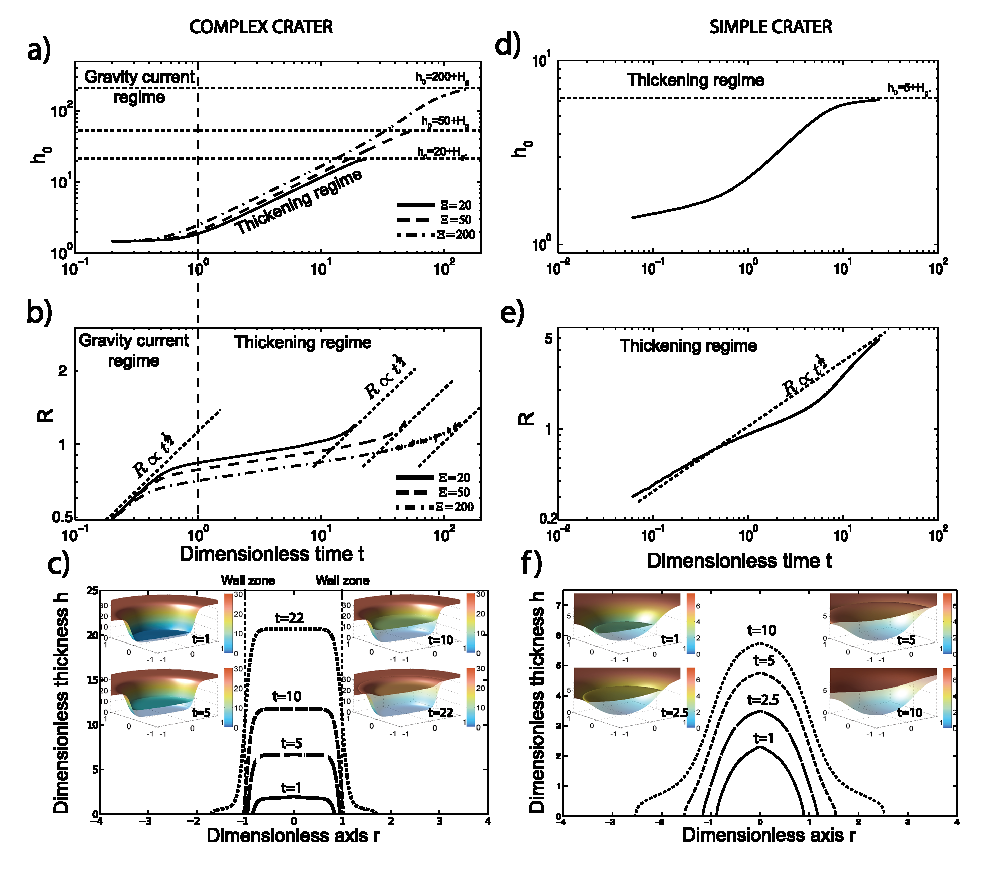
\includegraphics[scale=0.6]{fig4-2.eps}
  \caption{\textbf{a) and  b)}: Dimensionless thickness at  the center
    $h_0=h(0)$ and edge  radius $R$ versus dimensionless  time $t$ for
    the  case  of  an  intrusion  below  a  strengthless  layer,  i.e.
    $\Theta=0$,  with a  complex crater  topography and  for different
    values of  $\Xi$ indicated on  the graph.  Dimensional  values are
    obtained   by  multiplying   the  dimensionless   ones  by   their
    characteristic scales  i.e.  $C$,  $H$ (\ref{C5-eq18})  and $\tau$
    (\ref{C5-eq19}). The  vertical dashed  line indicates  $t=1$, when
    the intrusion reaches the wall zone. Horizontal dotted lines on a)
    represent  asymptotical  behaviors  for the  different  values  of
    $\Xi$.  On  b) The  dashed lines  $R\propto t^{1/2}$  indicate the
    scaling   law  in   the  gravity   current  regime.    \textbf{c)}
    Dimensionless intrusion profiles for  different times indicated on
    the  plot   using  $\Xi=20$.   For  each   time,  a  corresponding
    dimensionless 3D graph, showing the dimensionless floor appearance
    $T_p(r)+h(r)$,  where $T_p(r)$  is given  by (\ref{C5-TopoFinal}),
    superimposed  to   the  initial  dimensionless   floor  appearance
    $T_p(r)$  (low opacity),  is  represented to  see the  deformation
    induced  by   the  intrusion   on  the   crater  floor.    We  use
    $\gamma=0.02$,  $\zeta=0.13$ and  $\Theta=0$.  \textbf{d),  e) and
      f)} Same plots  but for an intrusion below  a strengthless layer
    with a simple crater topography, i.e. $\zeta=0.25$, using $\Xi=20$
    only. }
  \label{C5-fig4-2}
\end{figure}

Up to $t=1$,  the flow spreads as a classical  gravity current below a
flat floor  as the lithostastic term  (i.e.  second term on  the right
hand side of (\ref{C5-eq22})) is  negligible. In this regime, the flow
thickness goes  toward a  constant, noted $H_g$,  of order  $1$ (which
depends on  the source width \citep{Michaut:2009jx})  while the radius
evolves  as  $t^{1/2}$ as  predicted  by  the gravity  current  theory
\citep{Huppert:1982a}  (Figure \ref{C5-fig4-2}  a, b).   The intrusion
shows a  characteristic flat  top profile with  a steep  front (Figure
\ref{C5-fig4-2}  c).  When  the intrusion  reaches the  wall zone,  at
$t\sim1$,  the lithostatic  pressure increase  prevents the  intrusion
from  spreading   laterally.   The  second   term  on  the   right  of
(\ref{C5-eq22}) is  positive, it increases  with $\Xi$ and  causes the
thickening of  the intrusion (Figure  \ref{C5-fig4-2} a, c).   In this
thickening regime, the edge radius remains close to a constant (Figure
\ref{C5-fig4-2} b).   At the surface,  the thickening of the  flat top
intrusion results  in an  important piston-like  uplift of  the crater
floor. However,  no moat is formed  adjacent to the wall  zone (Figure
\ref{C5-fig4-2} c).
		 
In contrast to complex craters,  the topography of simple craters, and
hence the lithostatic pressure, gradually increases from the center to
the  exterior  of the  crater  wall  zone.   We use  $\zeta=0.25$  and
$\Xi=20$ in (\ref{C5-eq22}). In that case, there is no gravity current
phase;  the  gradual  lithostatic  pressure increase  slows  down  the
spreading from  the beginning and  induces a gradual  thickening phase
(Figure  \ref{C5-fig4-2}  d,  e,   f).   The  intrusion  shape  almost
accommodates  the  topography  (Figure  \ref{C5-fig4-2}  f).   Indeed,
because the overlying  layer is less dense than the  magma, the crater
floor appears slightly  concave up, the concavity  increasing with the
density difference between the overlying  layer and the magma, i.e. on
$\Omega$ (Figure \ref{C5-fig4-2} f).

For  both types  of craters,  the phase  of thickening  ends when  the
hydrostatic  pressure  due to  the  weight  of  the magma  equals  the
lithostatic pressure outside of the wall zone, i.e.  $h_{0} \sim \Xi$.
When  $h_{0} $  becomes larger  than $\Xi$,  the gravity  current term
compensates  for  the  lithostatic  term in  (\ref{C5-eq22})  and  the
intrusion can flow down the wall  zone and return in a gravity current
regime (Figure  \ref{C5-fig4-2} a, b,  d, e).  In the  gravity current
regime, the flow evolves toward a constant value equal to $\Xi + H_g$.
Thus, for a constant injection  rate, the number $\Xi$ mostly controls
the final intrusion  thickness and hence the shallowing  of the crater
floor.  However,  the injection rate  might decrease as  the intrusion
grows, as the intrusion weight compensates for the overpressure at the
origin  of  magma  ascent.   This  effect  should  control  the  final
shallowing  of   the  crater  floor   and  is  discussed   in  Section
\ref{C5-Injection_Rate}.
	
	
\subsection{Intrusion below an elastic layer of constant thickness}
\label{C5-Constant_Thickness}
		
In  the previous  section,  we considered  that  the intrusion  stalls
beneath   a   highly   fractured   and   brecciated   zone   with   no
strength. However, an impact melt unit  might be present on top of the
brecciated lens.  Furthermore, the intrusion might also emplace deeper
than the brecciated lens; both cases imply the deformation of an upper
coherent  elastic layer  during the  spreading of  the intrusion.   In
\citet{Michaut:2011kg}, the  model was developed for  an upper elastic
layer  of  constant thickness  in  a  2D  Cartesian geometry  and  the
behavior of the flow was predicted for an axisymmetric geometry. Here,
we  first show  the  results  for an  elastic  layer  with a  constant
thickness in  an axisymmetric geometry  and verify the  predictions of
\citet{Michaut:2011kg}. In the  next sections, we examine  the case of
an upper elastic  layer with a crater-like topography  and a thickness
that varies with the radius according to (\ref{C5-3-2}).

\begin{figure}[h!]
  \graphicspath{ {/Users/thorey/Documents/These/Submission/Article/FFC_JGR_2013/Paper_APRES_2nd_REVIEW/} }
  \centering
  \noindent\includegraphics[scale=0.6]{fig4-1.eps}
  \caption{\textbf{a) and  b)}: Dimensionless thickness at  the center
    $h_0=h(0)$ and edge  radius $R$ versus dimensionless  time $t$ for
    the  case  of an  intrusion  below  a constant  thickness  elastic
    layer. For $R<4$,  the flow dynamics is controlled  by the elastic
    deformation  of the  overlying layer,  while  for a  $R>4$, it  is
    controlled by its  own weight. In a), the  dashed lines correspond
    to  $h_{0}\propto t^{1/3}$  and $h_{0}  = H_g$  which provide  for
    scaling laws for  the elastic and gravity current  regimes.  In b)
    the  dashed  lines  $R\propto   t^{1/3}$  and  $R\propto  t^{1/2}$
    represent scaling laws for the elastic and gravity current regimes
    \citep{Michaut:2011kg}.   The vertical  dashed line  indicates the
    time when  the intrusion reaches  a radius of $4$.   The intrusion
    shape is shown at different times  in the elastic regime in c) and
    in  the  gravity current  regime  in  d).  We  use  $\gamma=0.02$,
    $\Xi=0$, $\Psi=0$ and $\Theta=1$. }
  \label{C5-fig4-1}
\end{figure}


We first solve Equation  (\ref{C5-eq21}) using $\Theta=1$, $\Xi=0$ and
$\Psi=0$,  i.e. $T_e(r)=T_{e}^0$  to model  the case  of a  magma that
flows beneath an  upper elastic layer of  constant thickness. Equation
(\ref{C5-eq21}) becomes:
		
\begin{eqnarray}
  \frac{\partial h}{\partial t}=\frac{1}{r} \frac{\partial}{\partial r}\left (rh^{3} \frac{\partial h}{\partial r} \right)+ \frac{1}{r}\frac{\partial}{\partial r}\left ( rh^{3} \frac{\partial}{\partial r}\left ( \nabla^{4}_{r}h \right )\right)+\frac{32}{\gamma^{2}} \left(\frac{1}{4}-\frac{r^{2}}{\gamma^{2}}\right)
  \label{C5-eq5.1}
\end{eqnarray}

In this case, there  is no limitation to the flow  as both the gravity
current term and the elastic term,  i.e. the first and second terms on
the right side of (\ref{C5-eq5.1}),  cause spreading. As expected, the
intrusion   dynamics   follows   two   different   spreading   regimes
\citep{Michaut:2011kg,Michaut:2013dr,Bunger:2011cb}.  During the first
phase,  the  thickening  is  important   and  the  intrusion  shows  a
bell-shaped  profile  (Figure  \ref{C5-fig4-1}  a, c).   As  shown  by
\citet{Michaut:2011kg}, the flow dynamics is controlled by the elastic
deformation of  the overlying  layer up to  a radius  $R=4\Lambda$. In
this regime, the elastic pressure is dominant over the pressure due to
magma weight. In the magma, the pressure is constant below the elastic
layer, except  at the tip  \citep{Bunger:2011cb,Michaut:2011kg}, which
explains   the   bell-shaped   profile  of   the   intrusion   (Figure
\ref{C5-fig4-1}  c). Indeed,  for  a constant  pressure  $P_d$ in  the
magma, $P_e(r)=D\nabla_r^4h=P_d$ implies
\begin{equation}
  h(r)=\frac{P_{d} R^{4}}{64D}\left(1-\left(\frac{r}{R}\right)^2\right)^2
  \label{C5-eq4-1}
\end{equation}
	
$D$ is the flexural rigidity of  the upper layer of constant thickness
as defined  by (\ref{C5-eq8a}).  Results  show that the  thickness and
radius evolve with time with an  exponent close to $1/3$, as predicted
by \citet{Michaut:2011kg} when neglecting the gravity current term and
considering  a  constant  injection rate  (Figure  \ref{C5-fig4-1}  a,
b). Beyond $R=4\Lambda$, the size of the intrusion becomes much larger
than  the  flexural  parameter  and  the  gravitational  term  becomes
prevalent in the dynamics. The intrusion thus transitions to a gravity
current   regime  characterized   by  a   flat  top   profile  (Figure
\ref{C5-fig4-1} d).  In this regime, the flow thickness evolves toward
a constant  $H_g$ while the  radius follows $t^{1/2}$ as  predicted by
the    gravity    current   theory    \citep{Huppert:1982a}    (Figure
\ref{C5-fig4-1} a, b). The elastic term is negligible when considering
the dynamics of the whole flow in this regime.  However, the overlying
layer is  unable to accommodate the  steep front of a  typical gravity
current flow \citep{Huppert:1982a} and  the intrusion develops a small
scale  bent   edge  whose  width   is  equal  to   $4\Lambda$  (Figure
\ref{C5-fig4-1} d).
		
\subsection{Spreading beneath a complex crater topography}
		
In this section,  we consider an intrusion below  an elastic overlying
layer with a  complex crater topography, hence we  use $\zeta=0.13$ in
(\ref{C5-eqqqq}).   We  first  examine   the  effect  of  varying  the
dimensionless  flexural  parameter,  i.e.   the  dimensionless  number
$\Theta$ and then examine the influence  of the thickening at the wall
by varying the number $\Psi$.
	
\subsubsection{Effect of the  dimensionless flexural parameter (effect
  of $\Theta$)}
		
We consider  equation (\ref{C5-eq21})  for which  we set  $\Xi=20$ and
$\Psi=0.3$  and consider  two  different values  of the  dimensionless
flexural  parameter  $\Theta=10^{-2}$  and  $\Theta=10^{-5}$.   Up  to
$t\sim1$, the  central flat  floor of  the crater  acts as  a constant
thickness upper  layer and  the lithostatic term  (second term  on the
right hand side of (\ref{C5-eq21})) is negligible.
	
For $\Theta=10^{-2}$, the  flexural wavelength is close  to the crater
size, i.e.   $4\Lambda \sim C$.   The intrusion spreads in  an elastic
regime  below the  crater  flat floor,  the  dimensionless radius  and
dimensionless   thickness   evolve    close   to   $t^{1/3}$   (Figure
\ref{C5-fig4-3}) and the intrusion  shows a characteristic bell-shaped
profile (Figure  \ref{C5-fig4-4} a). At  $t\sim1$, the second  term on
the right  hand side of (\ref{C5-eq21}),  representing the lithostatic
pressure  increase at  the  crater wall  zone,  becomes important  and
opposes to  the flow. The  intrusion enters in a  thickening dominated
regime,  where the  thickness increases  significantly and  the radius
remains close to constant  (Figure \ref{C5-fig4-3} and \ref{C5-fig4-4}
a), while  it has not yet  transitioned into a gravity  current regime
and  still shows  a bell  shape.   The thickening  of the  bell-shaped
intrusion  results in  a convex  uplift  of the  crater floor  (Figure
\ref{C5-fig4-4} a).
		
\begin{figure}[htpb]
  \graphicspath{ {/Users/thorey/Documents/These/Submission/Article/FFC_JGR_2013/Paper_APRES_2nd_REVIEW/} }
  \centering
  \noindent\includegraphics[scale=0.8]{fig4-3.eps}
  \caption{Dimensionless thickness  at the center $h_0=h(0)$  and edge
    radius  $R$ versus  dimensionless  time  $t$ for  the  case of  an
    intrusion  spreading  below  an  overlying elastic  layer  with  a
    topography characteristic of a  complex crater, i.e. $\zeta=0.13$,
    and  using  a constant  injection  rate.   Vertical dotted  lines:
    dimensionless  times  when the  intrusion  enters  and leaves  the
    thickening  regime.  Thick  solid  lines, $\Theta=10^{-2}$,  thick
    dashed  lines,  $\Theta=10^{-5}$.   Scaling   laws  are  shown  in
    dash-dotted  lines for  the  elastic  regime ($R\propto  t^{1/3}$,
    $h_0\propto t ^{1/3}$) and in dotted lines for the gravity current
    regime    ($R\propto    t^{1/2}$,     $h_0    \rightarrow    H_g$,
    $h_0 \rightarrow \Xi+ H_g$).  We use, $\gamma=0.02$, $\zeta=0.13$,
    $\Xi=20$ and $\Psi=0.3$.}
  \label{C5-fig4-3}
\end{figure}


For $\Theta=10^{-5}$, the intrusion first spreads in an elastic regime
and the dimensionless radius and thickness evolve as $t^{1/3}$ (Figure
\ref{C5-fig4-3}).  However,  the flexural  wavelength is  much smaller
than the crater  size in this case (i.e.  $4\Lambda  << C$).  The flow
transitions to a gravity current regime far in front of the wall zone,
at $t=0.06$, which is evident  as, beyond this time, the dimensionless
radius  evolves as  $t^{1/2}$ while  the dimensionless  thickness goes
toward a constant  (Figure \ref{C5-fig4-3} a and  b).  In consequence,
the intrusion  shows a flat  top profile and  a small scale  bent edge
while reaching  the crater wall  zone (Figure \ref{C5-fig4-4}  b).  At
$t\sim1$,  the lithostatic  pressure increase  prevents the  intrusion
from spreading radially and the  intrusion thickens. The thickening of
the flat top intrusion results in  a piston-like uplift of the central
part of the crater floor (Figure \ref{C5-fig4-3} a and \ref{C5-fig4-4}
b) as in  the previous case of a gravity  current below a strengthless
overlying layer  (Figure \ref{C5-fig4-2}  c). However, the  bending of
the upper layer above the intrusion at its edge leads to the formation
of  a  circular  moat,  adjacent   to  the  wall  zone,  whose  extent
corresponds to the  size of the intrusion edge and  is $\sim 4\Lambda$
(Figure \ref{C5-fig4-4} b).

\begin{figure}[h!]
  \graphicspath{ {/Users/thorey/Documents/These/Submission/Article/FFC_JGR_2013/Paper_APRES_2nd_REVIEW/} }
  \centering
  \noindent\includegraphics[scale=0.7]{fig4-4.eps}
  \caption{ \textbf{a) } Profiles for  an intrusion spreading below an
    elastic  overlying  layer  with  a complex  crater  topography  at
    different times  indicated on the plot  for $\Theta=10^{-2}$, i.e.
    corresponding to a small crater  and/or an intrusion below a thick
    elastic  layer.   Units  are  dimensionless.   For  each  time,  a
    corresponding  3D graph  showing  the  dimensionless crater  floor
    appearance  given  by $T_p(r)+h(r)$  where  $T_p(r)$  is given  by
    (\ref{C5-TopoFinal}),   is  represented.    For  each   plot,  the
    dimensionless initial  topography $T_p(r)$ is superimposed  in low
    opacity. \textbf{b)}  Same plot  but for a  large crater  and/or a
    shallow   intrusion,  i.e.    $\Theta=10^{-5}$.    Here,  we   use
    $\gamma=0.02$, $\zeta=0.13$, $\Xi=20$ and $\Psi=0.3$.}
  \label{C5-fig4-4}
\end{figure}

		 
The thickening  rate of the  intrusion, as  it reaches the  wall zone,
depends  on its  spreading regime  (Figure \ref{C5-fig4-3}  a, b)  and
hence on  the value of  $\Theta$. For  larger values of  $\Theta$, the
elastic pressure  that squeezes the flow  is more important and  it is
easier for  the magma to  overcome the lithostatic barrier  and spread
below the wall zone.   In any case, when the sum  of the pressures due
to  elastic  bending  of  the  overlying layer  and  to  magma  weight
compensates for the  hydrostatic pressure due to the  crater wall zone
weight, the flow passes the wall zone. For both values of $\Theta$, as
it passes  down the wall zone,  the intrusion is in  a gravity current
regime as $R$ is or becomes larger than $4\Lambda$: the radius evolves
as  $t^{1/2}$ and  the thickness  evolves  toward the  final value  of
$\Xi + H_g$ (Figure \ref{C5-fig4-3} a, b).
	
\subsubsection{Effect of the local  increase in the flexural parameter
  at the wall zone (effect of $\Psi$)}
		
Due to  the elastic thickness  increase at  the crater wall  zone, the
flexural  wavelength of  the  overlying elastic  layer increases  from
$\Lambda$ at the crater center to a value equal to
\begin{equation}
  \Lambda_{b}=\left( \frac{E(T_{e}^0+D_c)^3}{12(1-\nu^2)\rho_m g}\right)^{\frac{1}{4}} = \Lambda (1+\Psi)^{\frac{3}{4}}
\end{equation}
beyond the wall  zone. To understand the effect of  the local increase
in flexural wavelength at the wall  zone, we consider a constant value
of  the   number  $\Xi=20$  and   increasing  values  of   the  number
$\Psi=0.3,3,6$   for  the   two   different  values   of  the   number
$\Theta=10^{-2}$ and $\Theta=10^{-5}$ used previously and representing
two possible end-member floor deformations.
		
\begin{figure}[h!]
  \graphicspath{ {/Users/thorey/Documents/These/Submission/Article/FFC_JGR_2013/Paper_APRES_2nd_REVIEW/} }
  \centering
  \noindent\includegraphics[scale=0.7]{fig4-5.eps}
  \caption{   \textbf{a)}  Dimensionless   thickness  at   the  center
    $h_0=h(0)$ and edge radius $R$  versus dimensionless time $t$, for
    an intrusion  spreading below  an overlying  layer with  a complex
    crater topography,  for $\Theta=10^{-2}$  and different  values of
    $\Psi=0.3, 3$ and  $6$. The vertical dotted  lines indicate $t=1$,
    i.e.   the   time  at  which   the  intrusion  reaches   the  wall
    zone. \textbf{c)} Intrusion profiles for different times indicated
    on the  plot for $\Theta=10^{-2}$,  i.e. corresponding to  a small
    crater  and/or   a  deep   intrusion  and  $\Psi=6$.    Units  are
    dimensionless.   For each  time,  the corresponding  dimensionless
    crater floor appearance given  by $T_p(r)+h(r)$, where $T_p(r)$ is
    given by (\ref{C5-TopoFinal}), is represented.  For each plot, the
    dimensionless initial  topography $T_p(r)$ is superimposed  in low
    opacity.   \textbf{e)} Dimensionless  crater  floor appearance  at
    $t=10$ for $\Psi=6$, $\Theta=10^{-2}$. b), d) and f) Same plots as
    a), c)  and e)  but for  $\Theta=10^{-5}$.  We  use $\gamma=0.02$,
    $\zeta=0.13$ and $\Xi=20$.}
  \label{C5-fig4-5}
\end{figure}

For $\Theta=10^{-2}$,  the elastic term  is dominant over  the gravity
current term as  the flow arrives to  the wall zone and  the effect of
the local increase in flexural wavelength of the overlying layer is to
increase the thickening rate with time (Figure \ref{C5-fig4-5} a). The
increase in  flexural wavelength  enhances the  barrier effect  of the
lithostatic  pressure  increase  at  the  crater  wall  zone  and,  in
response, the flow  thickens rapidly in the center,  where the bending
is  easier (Figure  \ref{C5-fig4-5} a  and c).   The elastic  pressure
increases  with the  bending  and  after a  time  that increases  with
$\Psi$, it becomes important enough  to compensate for the lithostatic
pressure  increase at  the wall  zone and  induce a  squeezing of  the
intrusion below the  wall zone. For large values of  $\Psi$, the local
increase  in flexural  wavelength is  important at  the wall  zone and
forces the flow  to extend and deform the overlying  layer over a much
larger distance, beyond the crater,  than for smaller values of $\Psi$
(compare $\Psi=0.3$ and $6$ on Figure \ref{C5-fig4-5} a). As a result,
for  large  values  of  $\Psi$, the  intrusion  profile  relaxes,  the
thickness at the center collapses (Figure \ref{C5-fig4-5} a and c) and
the radius increases quickly. After the relaxation of the profile, the
intrusion  is  still in  an  elastic  regime  but characterized  by  a
flexural parameter $\Lambda_b$. Once  the dimensionless radius reaches
$r=4\Lambda_{b}/C=
4\Lambda(1+\Psi)^{3/4}/C=4\Theta^{1/4}(1+\Psi)^{3/4}$,
the  intrusion  transitions to  a  gravity  current regime  where  the
thickness evolves toward a constant  and the radius grows as $t^{1/2}$
(Figure  \ref{C5-fig4-5}   a).   For   instance,  for   $\Psi=3$,  the
transition    to    a    gravity   current    regime    occurs    when
$R= 4\Theta^{1/4}(1+\Psi)^{3/4}=3.6$ (Figure \ref{C5-fig4-5} a).
	 
For $\Theta=10^{-5}$,  the gravity current  term is dominant  when the
intrusion reaches the wall zone and the elastic term only controls the
shape of the  front (Figure \ref{C5-fig4-5} b and d).   And hence, the
thickening rate only increases by a few percent between $\Psi=0.3$ and
$\Psi=6$,  while it  increases  by a  factor  of $3$  in  the case  of
$\Theta=10^{-2}$ (Figure \ref{C5-fig4-5} a  and b).  Nevertheless, the
local increase in the flexural wavelength below the wall zone tends to
enlarge  the size  of the  intrusion edge  and to  result in  a deeper
circular moat at the surface (Figure \ref{C5-fig4-5} d and f).
		 
\subsection{Spreading beneath a simple crater}
\label{C5-SimpleCrater}
		
In comparison to complex craters,  the lithostatic pressure as well as
the flexural wavelength of the upper layer gradually increase from the
center to the exterior of the  crater wall zone. Given the appropriate
range of  values for the  number $\Theta=10^{-3}-10$, as  discussed in
Section  \ref{C5-Dimensionless_Number},  the   flexural  parameter  is
between $0.2$ and $1$ times the  crater radius $C$. The bending of the
upper layer thus controls the  intrusion shape and dynamics during the
whole  flow and  the intrusion  always  shows a  bell shaped  geometry
(Figure \ref{C5-fig4-6}).  To represent the case of an intrusion below
a bowl-shaped crater, we use $\zeta=0.25$, $\Xi=20$, $ \Theta=0.1$ and
we  study the  effect of  the  thickening at  the wall  zone by  using
different values of $\Psi=0.1$ and $\Psi=4$.

\begin{figure}[h!]
  \graphicspath{ {/Users/thorey/Documents/These/Submission/Article/FFC_JGR_2013/Paper_APRES_2nd_REVIEW/} }
  \centering
  \noindent\includegraphics[scale=0.6]{fig4-6.eps}
  \caption{  \textbf{a)}  Dimensionless   profiles,  of  an  intrusion
    spreading below  an overlying elastic  layer with a  simple crater
    topography, i.e.  $\zeta=0.25$,  for different dimensionless times
    indicated  on the  plot for  $\Theta=10^{-1}$ and  $\Psi=0.1$. For
    each  time, a  corresponding 3D  graph, showing  the dimensionless
    crater floor appearance given  by $T_p(r)+h(r)$, where $T_p(r)$ is
    given by (\ref{C5-TopoFinal}), is represented.  For each plot, the
    initial  topography  $T_p(r)$  is  superimposed  in  low  opacity.
    \textbf{b)} Same plot but for $\Psi=4$.  We use, $\gamma=0.02$ and
    $\Xi=20$.}
  \label{C5-fig4-6}
\end{figure}
		
For $\Psi=0.1$,  the thickening  at the  wall zone  $\Psi \xi(r)  $ is
negligible  and the  elastic term  is similar  to that  of a  constant
thickness  layer.  However,  the lithostatic  pressure increase  slows
down the spreading and the evolution of the radius with time is slower
than  for an  elastic regime  below a  constant thickness  layer.  The
intrusion  shows a  bell-shaped  profile with  an important  curvature
because the weight of the lithostatic barrier constrains the intrusion
edge  (Figure \ref{C5-fig4-6}  a).  For  $\Psi=4$, the  local flexural
wavelength rapidly rises up to $\Lambda_{b}=\Lambda(1+\Psi)^{3/4}$. As
a consequence, the  intrusion squeezes more rapidly  and thickens more
slowly  than  for smaller  values  of  $\Psi$ (Figure  \ref{C5-fig4-6}
b). For a larger value of $\Psi$, the deformation occurs over a larger
wavelength and  the shallowing is  smaller at a given  time.  However,
the overall deformation at the surface  is very similar in both cases:
the crater floor appears convex and shows an important curvature which
overlaps the initial bowl shape  of the crater (Figure \ref{C5-fig4-6}
a, b).
	 
\subsection{Effect of a variable injection rate}
\label{C5-Injection_Rate}
	 
So  far, we  have assumed  a constant  injection rate;  and hence  the
intrusion grows indefinitely in volume  and the flow passes the crater
wall zone.  However, the driving pressure in the feeder conduit should
decrease  as the  intrusion  grows during  the  thickening phase.   In
particular, the increase  in hydrostatic pressure due  to magma weight
and in  elastic pressure due to  bending above the dyke  might finally
compensate for the initial overpressure $\Delta P$ in the magma at the
origin of  the flow.  As the  increase in lithostatic pressure  at the
crater wall zone prevents the  intrusion from spreading laterally, the
intrusion might reach  a steady state profile such that  no more magma
can intrude. New  expressions for the vertical  injection velocity and
injection rate,  taking into account  the increase in pressure  in the
magma at the top of the feeder dyke, are given by:
\begin{equation}
  w(r,t)=\frac{32}{\gamma^{2}} \left(1-\frac{1}{\sigma}\left(h_0+P_{e,r=0} \right)\right)
  \left(\frac{1}{4}-\frac{r^{2}}{\gamma^{2}}\right)
  \label{C5-5.3}
\end{equation}
and
\begin{equation}
  Q_{0}=\left(1-\frac{1}{\sigma}\left(h_0+ P_{e,r=0}\right)\right)
  \label{C5-eq5.4}
\end{equation}
where
\begin{equation}
  \sigma=\frac{\Delta P}{\rho_{m}gH}
  \label{C5-eq5.4.5}
\end{equation}
and
\begin{equation}
  P_{e,r=0}= \Theta \nabla^{2}_{r}\left.\left ((1+\Psi \xi(r))^{3}\nabla^{2}_{r}h \right )\right|_{r=0}
\end{equation}
The dimensionless  number $\sigma$ represents the  normalized pressure
head, $P_{e,r=0}$ is the dimensionless  elastic pressure at the center
and $Q_{0}$ the  dimensionless total injection rate.   As discussed in
\citet{Michaut:2011kg}, the  elastic pressure $P_{e,r=0}$  required to
bend  the upper  layer  tends  to infinity  as  $R\rightarrow 0$,  but
rapidly decreases with the radius as $P_{e,r=0}$ scales with $h_0/R^4$
(see (\ref{C5-eq8})). However, here we assume a large aspect ratio for
the  intrusion (lubrication  assumption), and  this initial  transient
regime, where the  flow is very narrow and $P_{e,r=0}$  is very large,
is  thus   not  representative   of  the   initiation  phase   of  the
intrusion. Hence, to investigate the effect of the elastic pressure on
the injection rate, we neglect this initial transient phase.

\begin{figure}[h!]
  \graphicspath{ {/Users/thorey/Documents/These/Submission/Article/FFC_JGR_2013/Paper_APRES_2nd_REVIEW/} }
  \centering
  \noindent\includegraphics[scale=0.65]{fig4-7a.eps}
  \caption{\textbf{a)}  Dimensionless   pressure  in  the   magma  $P$
    normalized by the value of  $\sigma$ versus dimensionless time $t$
    for $\Theta=10^{-2}$, for an  intrusion spreading below an elastic
    overlying layer with a complex  crater topography.  The solid line
    represents the  dimensionless pressure at  the center of  the flow
    normalized              by              $\sigma$,              i.e
    $P_{tot}/\sigma=(h_0+P_{e,r=0})/\sigma$, the dashed line indicates
    the  magma  weight  contribution $P_m/\sigma=h_0/\sigma$  and  the
    dash-dotted  line  represents  the elastic  pressure  contribution
    $P_{e,r=0}/\sigma$.   The  vertical   dotted  line  indicates  the
    dimensionless  time  when the  intrusion  reaches  the wall  zone.
    \textbf{b)} Initial  (dashed line) and final,  i.e.  steady state,
    (solid line)  dimensionless topography of the  crater. \textbf{c)}
    and \textbf{d)} Same plots as  \textbf{a)} and \textbf{b)} but for
    $\Theta=10^{-5}$.  In  c), the dashed line  representing the magma
    weight  contribution   is  not  distinguishable  from   the  total
    pressure.   For  all  plots,  horizontal  dotted  lines  represent
    asymptotic   behaviors.     We   use    $\gamma=0.02$,   $\Xi=50$,
    $\zeta=0.13$, $\Psi=1$ and $\sigma=22$.}
  \label{C5-fig4-7}
\end{figure}
 
Given that  the deformations  are limited to  craters, it  is possible
that  excavation of  material  during the  impact  has controlled  the
intrusion of magma.  In that case,  the driving pressure $\Delta P$ at
the origin of the flow should be lower or equal to the weight of crust
that has been  removed by cratering, i.e.  $\Delta  P\le \rho_c gD_c$,
which implies $\sigma<\Xi$ (see (\ref{C5-n3}) and (\ref{C5-eq5.4.5})).
Hence,  given   the  range  of   values  for  the   parameters  (Table
\ref{C5-tab2}), the value of the  number $\sigma$ varies between $0.6$
and $100$  (Table \ref{C5-tab3}).  We  consider a complex  crater with
$\zeta=0.13$ and we set $\Xi=50$, $\Psi=1$, $\sigma=22$ and two values
of $\Theta$, equal to $10^{-2}$  and $10^{-5}$, to consider the effect
of a variable injection rate.

For $\Theta=10^{-2}$,  the elastic  pressure governs the  spreading of
the intrusion below the crater  flat floor; as $P_{e,r=0}$ scales with
$h_0/R^4$, $P_{e,r=0}$  decreases as the  flow spreads and  its radius
increases (Figure \ref{C5-fig4-7} a) inducing an increase in the total
injection  rate  $Q_{0}$  (\ref{C5-eq5.4}).  Then,  as  the  intrusion
thickens,  both the  pressure  due  to magma  weight  and the  elastic
pressure increases at the  center, in response (Figure \ref{C5-fig4-7}
a). The total injection rate decreases and the system reaches a steady
state   shape  when   $Q_{0}\rightarrow0$,   i.e   when  the   initial
overpressure is compensated by the sum  of the elastic pressure and of
the pressure due to magma weight (Figure \ref{C5-fig4-7} a,b).

For  $\Theta=10^{-5}$,  the  weight  of  the  magma  is  the  dominant
contribution  to  the  pressure  during  the  whole  flow  ($P_m$  and
$P_{tot}$ are not distinguishable on Figure \ref{C5-fig4-7} c) and the
injection rate remains close to a constant while the intrusion spreads
below  the crater  flat  floor  in a  gravity  current regime  (Figure
\ref{C5-fig4-7} c).   As the intrusion  thickens, the weight  of magma
increases  at  the center  (Figure  \ref{C5-fig4-7}  c) leading  to  a
decrease  in   the  total  injection  rate   (\ref{C5-eq5.4}).   When,
$h_{0}=\sigma=22$,  no  more  magma  intrudes below  the  crater,  the
intrusion thickness as well as the radius stabilized and the intrusion
reaches its steady state shape (Figure \ref{C5-fig4-7} c, d).

The normalized pressure head thus controls the amount of shallowing of
the crater  floor. If the pressure  head is larger than  the weight of
the crust that has been removed by cratering, the intrusion would pass
the  wall zone  and reach  a constant  thickness, but  it would  still
continue to flow laterally beyond the wall zone (see lateral spreading
regime in \citet{Michaut:2011kg}).  In  contrast, if the pressure head
is  less  than the  weight  of  the crust  that  has  been removed  by
cratering, the intrusion reaches a steady-state shape and deformations
are constrained within  the crater. In that case, for  small values of
$\Theta$, the amount of shallowing is directly the normalized pressure
head  $\sigma$ while  for  relatively large  values  of $\Theta$,  the
intrusion   reaches   a  steady   state   profile   for  a   thickness
$h_{0}\le \sigma$.
	
	
\section{Discussion}

\subsection{Floor appearance}
	
Viscous relaxation tends to  relax large wavelength structures without
affecting or  creating small-scale  features.  In  particular, viscous
relaxation is not able to explain  the presence of moats bordering the
wall    region    observed    in    different    classes    of    FFCs
\citep{Schultz:1976kt,Jozwiak:2012dq}.  Relaxation of the crater floor
also tends to  produce a convex profile at the  end of the deformation
\citep{Dombard:2001gs}  and cannot  account  for  central flat  floors
observed for FFCs of class $3$ and $5$ \citep{Jozwiak:2012dq}.
	
In contrast,  our model is  able to  reproduce the different  kinds of
floor appearances observed  at FFCs and thus  confirms the predictions
initially made by \citet{Schultz:1976kt}.   In particular, for a given
crater  size, the  thickening caused  by the  increase in  lithostatic
pressure at the crater wall zone induces either a convex uplift of the
crater floor, if the intrusion occurs  below a thick elastic layer, or
a piston-like uplift of the crater floor if the intrusion occurs below
a  strengthless and  highly brecciated  zone or  below a  thin elastic
layer. This  piston-like uplift  results in  a large,  shallowed plate
like floor as predicted by \citet{Schultz:1976kt}.
	
In addition, the  model shows that the final appearance  of the crater
floor is  controlled by the  ratio between the flexural  wavelength of
the  overlying  layer,  that  mainly  depends  on  the  elastic  layer
thickness,   and    the   crater    size,   i.e.    on    the   number
$\Theta=(\Lambda/C)^4$.   Indeed,  because   the  deformation  of  the
overlying elastic layer  is accommodated along a  width of $4\Lambda$,
our model  predicts a  transition between  a flat  floor and  a convex
floor  when $4\Lambda\sim  C$, i.e.   at $\Theta=10^{-3}$.   For large
values of $\Theta>10^{-3}$, i.e. small  craters and/or a thick elastic
layer overlying the intrusion, the  bending of the upper elastic layer
affects  the whole  crater width  resulting in  a convex  crater floor
(Figure \ref{C5-fig4-4} a).  On the contrary, for large craters and/or
a thin  elastic layer overlying  the intrusion, i.e.  small  values of
$\Theta<10^{-3}$, the thickening of the  flat top intrusion results in
a flat central floor with a circular moat that borders the interior of
the wall zone  (Figure \ref{C5-fig4-4} b). This  circular moat results
from the elastic  deformation of the overlying layer  at the intrusion
front and its size is equal  to $4\Lambda$.  Finally, if the overlying
layer is strengthless and $\Theta=0$, the crater floor appears flat or
slightly  concave up  because of  the density  difference between  the
magma and the overlying layer.
	
FFCs  of classes  3 and  5 show  a central  uplifted flat  floor; they
generally have a  large diameter: the mean diameter is  of $50$ km for
craters  of class  3, and  $70$  km for  craters of  class $5$  (Table
\ref{C5-tab1})  \citep{Schultz:1976kt,Jozwiak:2012dq}.    These  large
diameters are coherent  with a small value  of $\Theta$ (\ref{C5-n5}),
i.e.  with  an intrusion in the  gravity current regime as  it reaches
the wall  zone and a piston-like  uplift of the central  flat floor of
the crater.  A moat bordering the  wall region is observed for craters
of class 3 in agreement with  our results for small values of $\Theta$
(see for instance the topography  of FFC Warner Figure \ref{C5-fig5-1}
b).  Craters of class 5 have a central shallowed flat floor but do not
show  a moat  bordering the  wall region  (Table \ref{C5-tab1}).   One
possibility is  that the intrusion  has emplaced below  a strengthless
layer.  Another possibility is that  these craters have been partially
infilled before deformation by basin ejecta \citep{Schultz:1976kt}; as
a  result,  the  thickening  of  the intrusion  was  limited  and  not
important  enough to  form  a moat.   Furthermore,  for large  craters
and/or intrusions below a thin  elastic layer, our model predicts that
the maximum stresses are concentrated upon the intrusion edge within a
crown  bordering the  wall  region (Figure  \ref{C5-fig7-1} c).   This
stress  concentration in  front of  the crater  wall could  induce new
fractures or  reactivate preliminary  fractures caused by  the impact,
providing  privileged paths  for  the  magma to  rise  to the  surface
\citep{Schultz:1976kt}.   Indeed,   pyroclastic  deposits   have  been
observed  in   floor-fractured  craters   of  classes  $3$   and  $5$,
preferentially  located within  fractures  adjacent to  the wall  zone
\citep{Schultz:1976kt}.
	 
Convex  floors characterize  FFCs  of  classes $2$  and  $4$ (see  for
instance FFC Briggs, Figure \ref{C5-fig5-1}  a).  Craters of classes 2
and 4  are in fact generally  small; their average diameters  are $30$
and  $20$ km  respectively  \citep{Jozwiak:2012dq} with  some of  them
being initially simple craters (Table \ref{C5-tab1}); this is coherent
with  large values  of $\Theta$  and a  final convex  floor appearance
according to our model. In FFCs of  class 4, a more or less pronounced
narrow V-shaped moat is observed adjacent  to the wall zone as well as
pronounced inner ridges  for FFCs of class  4 b.  In the  frame of our
model, we can  interpret these features as resulting  from the rupture
of the  upper layer  during the thickening  regime. Indeed,  our model
predicts that  the radial stress  might not  be maximum at  the crater
center, even  for a  convex floor,  but at  a given  radial coordinate
$r_{\sigma_{max}}$  such  that  $0<r_{\sigma_{max}}<1$  (see  Appendix
\ref{C5-AppendixB}, Figure \ref{C5-fig7-1} a, b) because the intrusion
might transition from an elastic to a gravity current shape before the
wall zone and because the elastic thickness increases towards the wall
zone. The  location of $r_{\sigma_{max}}$  depends on time and  on the
values  of  $\Theta$  and  $\Psi$. This  location  of  maximum  stress
provides a  preferred location for  a concentric failure of  the upper
elastic layer.
	 
Furthermore, our  model can also explain  the variable characteristics
of central peaks of FFCs \citep{Schultz:1976kt}.  In the case where an
elastic layer  is present,  our model predicts  that the  central peak
would  be leveled  up  during  the uplift  and  slightly smaller  than
initially  (see  Appendix \ref{C5-AppendixC},  Figure  \ref{C5-fig7-2}
b,c).  \citet{Schultz:1976kt} indeed observed that there is a tendency
for central peaks of FFCs to  be smaller than those for well-preserved
impact  craters.   Furthermore,  a  small circular  moat  borders  the
central  peak  if   this  elastic  layer  is   relatively  thin,  such
$4\Lambda<C$ (see Appendix  \ref{C5-AppendixC}, Figure \ref{C5-fig7-2}
b). The build up of stress resulting from the flexure within this moat
could be coherent  with the fracture pattern observed  in the vicinity
of central peaks at some FFCs \citep{Schultz:1976kt}.  Finally, if the
layer overlying  the intrusion is  formed by incoherent  breccias, the
central peak  would be buried during  the uplift, or its  initial size
significantly reduced  if the shallowing  is smaller than  the central
peak height,  and could  thus be  absent from  the uplifted  floor, as
observed  in   a  few   cases  \citep{Schultz:1976kt}   (see  Appendix
\ref{C5-AppendixC}, Figure \ref{C5-fig7-2} a).
		 
\subsection{Depth of the intrusion}
		
The deformation of a layer overlying a shallow magmatic intrusion such
as a laccolith  has been classically modeled by  the upward deflection
of a thin  elastic layer submitted to the pressure  $P_{d}$ within the
intrusion  (\ref{C5-eq4-1}).   In  this  kind  of  static  model,  the
internal pressure $P_{d}$  within the intrusion is  usually assumed to
be a constant and equal to  the hydrostatic pressure due to the weight
of the  magma at the  center of the  intrusion.  The solution  to this
problem  gives  a floor  deflection,  or  maximum intrusion  thickness
$h_0$,  that  varies  with   radius  to  the  fourth  (\ref{C5-eq4-1})
\citep{Johnson:1973ho,Pollard:1973ho}.   In the  case of  an intrusion
below the  floor of  a crater,  the crater  radius clamps  the elastic
overlying layer  and the intrusion  radius can be considered  equal to
the  crater  radius,  if  the deformation  affects  the  whole  crater
floor. And hence, this approach has motivated many previous studies to
derive  the intrusion  depth  from  the estimated  uplift  at a  given
floor-fractured crater \citep{Wichman:1996bj,Jozwiak:2012dq}.
		
However, there  is an  inconsistency in equating  the pressure  due to
magma weight  and the elastic  pressure deforming the  overlying plate
since both pressures act in favor of flow spreading. Assuming that the
final steady-state shape  of the flow has been reached,  i.e. that the
intrusion has  reached the wall zone  and that the pressure  above the
feeding conduit is equal to  the initial overpressure driving the flow
in  the conduit  (see Section  4.4), and  assuming that  the overlying
elastic layer making  the crater floor has a constant  thickness up to
the wall zone,  the function (\ref{C5-eq4-1}) may  indeed describe the
vertical  displacement  of  the  overlying layer  due  to  an  elastic
pressure  $P_{e}$.  But  this  is  true only  in  the  case where  the
intrusion is  in the elastic regime,  i.e. if the elastic  pressure is
dominant over the  pressure due to magma weight and  in this case, the
pressure necessary for  deforming the overlying plate  $P_{e}$ is then
not supported by  magma weight but by the driving  pressure within the
feeding dyke (see  \citep{Michaut:2011kg}, Section 6.1).  Furthermore,
if the  thickening at the wall  zone is significant, the  curvature of
the intrusion is accentuated by the interaction with the wall zone and
(\ref{C5-eq4-1}) is not accurate anymore.  Moreover, for large craters
or shallow intrusions, i.e.  $4\Lambda  <C$, the intrusion lies in the
gravity current regime  when it reaches the crater wall  zone. In that
case, the dominant pressure comes  from magma weight and, assuming the
intrusion has reached  the wall zone and its  steady-state shape, then
the overpressure driving the injection  is compensated by magma weight
and, $P_{d}=\rho_{m}gh$ is a good  estimate of the pressure within the
flow. However in  this case, the intrusion is characterized  by a flat
top  and its  profile  is very  different  from (\ref{C5-eq4-1})  (see
Section   4.2.2)   \citep{Bunger:2011cb,Michaut:2011kg}   and   hence,
(\ref{C5-eq4-1}) is no longer accurate to derive the intrusion depth.
		
Finally,  using (\ref{C5-eq4-1})  and equating  $P_d=\rho_m g  h_0$ to
derive the intrusion depth $T_e^0$ at FFCs leads to an intrusion depth
that scales with the crater diameter to the power four third, i.e. the
larger the crater, the deeper the  intrusion.  But, there is no reason
to suppose that the intrusion depth scales with the crater size.
		
In contrast, the model we develop provides a simple method to estimate
the elastic  thickness of the  layer overlying the intrusion  from the
floor appearance.  As  discussed above, the floor of  a crater appears
convex if the flexural wavelength of the layer overlying the intrusion
is  such that  $4  \Lambda \ge  C$.  As  $\Lambda$  mainly depends  on
$T_{e}^0$,  and assuming  the intrusion  has reached  the crater  wall
zone,  this inequality  provides  for  a lower  bound  on the  elastic
thickness of the upper layer:
		 
\begin{equation}
  T_{e}^0 \ge \left(\frac{12(1-\nu^{2})\rho_{m}gC^{4}}{4^4 E}\right)^{1/3}
  \label{C5-eq5-2}
\end{equation}

For instance, Briggs is a class 2 FFC of 37 km in diameter, it shows a
large convex floor (Figure \ref{C5-fig5-1} a).  Hence (\ref{C5-eq5-2})
applies and  we estimate  that the intrusion  lies beneath  an elastic
layer whose  thickness is equal  to or deeper  than $1.6$ km  for this
specific   crater,   using   parameter    values   listed   in   Table
(\ref{C5-tab2}). This value is only  a minimum value for the intrusion
depth, as  it does not take  into account the potential  presence of a
brecciated layer on top or below the elastic layer.
		
In the case of a crater showing a flat floor with a circular moat, the
intrusion should be in a gravity  current regime, and, assuming it has
reached  the  wall  zone (which  is  likely  to  be  the case  if  the
shallowing  is  significant), then  the  width  of the  moat  directly
provides for an  estimate of the flexural wavelength  of the overlying
elastic layer, and hence for  the elastic thickness.  Indeed, the size
of the moats  corresponds to the width of the  intrusion edge, i.e. to
$4\Lambda$ (see Figure \ref{C5-fig4-1} d, Figure \ref{C5-fig4-4} b and
Section \ref{C5-Constant_Thickness}).   For instance, for the  class 3
FFC Warner,  which is  $35$ km  in diameter,  the deformation  shows a
plate-like central flat  floor, with a moat bordering  the wall region
of about  one third of  the crater radius (Figure  \ref{C5-fig5-1} b).
Hence, $(4\Lambda)/C\sim 1/3$ and the elastic thickness $T_e^0$ varies
between $300$  and $600  $ m.Again, this  estimate provides  a minimum
value for the intrusion depth.
			
\subsection{Injection rate and formation time scale}
\label{C5-InjectionRateDiscussion}
		
Precedent works have shown that, for  craters smaller than $100$ km in
diameter, the  shallowing associated with viscous  relaxation is small
or almost  inexistent \citep{Dombard:2001gs}.  In contrast,  our model
of magmatic  intrusion is able  to reproduce the large  discrepancy in
crater floor shallowing observed at FFCs. Two mechanisms might control
the final amount of shallowing: the  injection rate and the cooling of
the intrusion.
		
If the  cooling time scale of  the intrusion is large  compared to its
formation time  scale, then  the intrusion reaches  the wall  zone and
thickens.   In that  case,  assuming a  constant  injection rate,  the
maximum amount  of shallowing  corresponds to the  intrusion thickness
that  evolves  toward  a  dimensionless  thickness  of  $\Xi  +  H_g$.
However,   as  explained   in  Section   \ref{C5-Injection_Rate},  the
injection rate should  decrease as the intrusion  grows, in particular
during the thickening phase.  Indeed,  when the magma reaches the wall
zone, the pressure  due to magma weight and to  elastic deformation of
the  overlying layer  increases as  the crater  floor is  uplifted and
might finally compensate for the  initial pressure driving the flow in
the  melt source.   An estimate  of this  initial overpressure  can be
derived from  our model in  some cases.   Indeed, for small  values of
$\Theta$,  i.e. for  craters  that show  a flat  floor  like those  of
classes $3$  and $5$,  the overpressure  in the  melt source  might be
estimated  from the  final thickness  of the  intrusion at  the center
$h_0^f$,   i.e.    $\Delta    P=\rho_{m}gh_{0}^f$   as   proposed   by
\citet{Jozwiak:2012dq}  (Figure \ref{C5-fig4-7}  c,  d). However,  for
large values of $\Theta$, i.e.  for  craters that show a convex floor,
as craters of classes $2$ and $4$, this assumption is inappropriate as
both  the  pressure due  to  magma  weight  and the  elastic  pressure
contribute to compensate for the initial overpressure $\Delta P$, i.e.
$\Delta P> \rho_m gh_0^f$ (Figure \ref{C5-fig4-7} a and b).
	
For most  FFCs, the deformation  is contained within the  crater floor
\citep{Schultz:1976kt} suggesting that the  removal of material during
the impact  controlled the  initial overpressure  in the  melt source.
However, impact craters commonly show  a raised rim, which is uplifted
relative  to the  pre-impact  surface and  this  structure could  also
contribute to prevent the intrusion from growing beyond the wall zone.
Finally, in a few cases such as crater Haldane \citep{Schultz:1976kt},
the deformations extend well beyond the wall zone and suggest that the
intrusion passed  the wall zone,  i.e.  that the  initial overpressure
might have  been larger than  $\rho_c g D_c  +P_r$ where $P_r$  is the
lithostatic pressure excess induced by the raised rim.
		
The deep  floor of  Class 1  FFCs suggests  that these  craters didn't
undergo  the thickening  phase  (Table  \ref{C5-tab1}).  However,  the
network of fractures on their floor  is coherent with the spreading of
an  underlying intrusion  that might  be an  aborted sill  that cooled
before reaching the  wall zone.  In that case, the  time scale for the
intrusion to  reach the wall  zone $\tau=(\pi C^2 H)/Q_{0}$  is larger
than the time scale for cooling  of the intrusion.  The time scale for
cooling can be  estimated from the characteristic  time for conductive
cooling of an intrusion of average thickness $\bar{h}$
\begin{equation}
  \tau_{c}= \frac{\bar{h}^{2}}{\pi\kappa}
  \label{C5-diff}
\end{equation}
where $\kappa=10^{-6}$ m$^{2}$.s$^{-1}$ is  the thermal diffusivity of
basalt. For large  craters of class $1$, the intrusion  is more likely
to be in  a gravity current regime with an  average thickness close to
$\bar{h}\sim2H$.  The inequality  $\tau_{c} \le \tau$ ((\ref{C5-eq19})
and  (\ref{C5-diff})) provides  for  an upper  bound  for the  average
injection rate:

\begin{equation}
  Q_{0}\le408 (C^{8}\kappa^{4}\rho_{m}g)^{\frac{1}{5}}
  \label{C5-eq5-3}
\end{equation}

For instance, for  the crater Atlas, which is $87$  km in diameter and
is located  at 46.7。N, 44.4。E in  the southeast of Mare  Frigoris, the
injection  rate should  be  smaller  than $10^{-2}$  m$^{3}$.s$^{-1}$,
using parameter values listed in  Table (\ref{C5-tab2}). This value is
for instance in agreement with the extrusion rate of lavas on the Moon
estimated  at the  end of  the  Imbrian and  during the  Eratosthenian
period  by  \citet{Head:1992bk}.   However,  most  of  the  FFCs  have
undergone   a    thickening   stage   and   hence    are   such   that
$\tau_{c} \ge  \tau$, and this  inequality provides for a  lower bound
for the average injection rate for these craters.
 		
\section{Conclusion}
		
The model  shows that the spreading  of an intrusion at  depth below a
crater is able to reproduce the deformations observed at FFCs and thus
confirms the different predictions made by \citet{Schultz:1976kt}.  In
particular,  the  increase in  lithostatic  pressure  and in  flexural
wavelength of the overlying layer at  the crater wall zone prevent the
intrusion  from spreading  radially  and induce  a  thickening of  the
intrusion that leads  to the shallowing of the crater  floor. When the
time scale for  conductive cooling of the intrusion  is large compared
to the formation time scale, the amount of shallowing is controlled by
the initial overpressure  in the melt source. The  model predicts that
the   final   appearance   of   the  crater   floor,   including   the
presence/disappearance of a central peak,  is mainly controlled by the
upper  layer flexural  wavelength $\Lambda$,  i.e.  its  structure and
thickness, and the crater radius $C$.
	
For an  overlying layer with  no elastic strength, i.e.   an intrusion
emplaced within or  immediately beneath a brecciated  lens, the crater
floor is flat at the end of  the deformation. If an elastic layer lies
on  top  of  the  intrusion,   but  is  sufficiently  thin  such  that
$C\ge 4\Lambda$, the crater shows a central plate-like floor separated
from the  wall zone by  a circular moat.   This moat results  from the
deformation of  the thin elastic  overlying layer above  the intrusion
front and its width  is equal to $4\Lambda$. The depth  of the moat is
controlled by the  amount of thickening of the overlying  layer at the
crater wall  zone.  Finally,  if the intrusion  is emplaced  beneath a
thick elastic layer such that $C< 4\Lambda$, the crater shows a convex
floor.

Within the framework of this model,  FFCs of class 1 would result from
aborted sills that have cooled  before reaching the wall zone. Craters
showing a convex floor, such as those of classes 2 and 4, would result
from the  spreading of an  intrusion below a relatively  thick elastic
layer, such that $\Lambda \ge C/4$. On the contrary, craters showing a
flat floor, such  as those of classes  3 and 5, would  result from the
spreading of  an intrusion  beneath a  relatively thin  elastic layer,
such that $\Lambda <<C/4$. The wide  circular U-shaped moat of class 3
FFCs is well explained by the  elastic deformation of the thin elastic
layer overlying the intrusion while the V-shaped moat of class 4 FFCs,
showing  a convex  floor, could  be explained  by the  rupture of  the
overlying layer,  which is predicted  to occur at a  radial coordinate
intermediate between  the center and the  wall zone. The absence  of a
moat for craters of class 5  could suggest that the intrusion develops
immediately beneath or within a breccia lens and that not sufficiently
impact   melt  stands   above   the  breccia   to   form  an   elastic
layer. Finally, class 6 FFCs are  filled up by lavas that have reached
the surface.
	
In addition,  the model allows  to constrain the elastic  thickness of
the layer lying on top of  the intrusion, which provides a lower bound
for the intrusion depth.

%%% Local Variables:
%%% mode: latex
%%% TeX-master: "../main"
%%% End:
